\documentclass[12pt]{article}

\usepackage{sbc-template}
\usepackage{graphicx,url}
\usepackage[brazil]{babel} 
\usepackage[utf8]{inputenc}
\usepackage{comment}
\usepackage{microtype}
\usepackage[hidelinks,hyperindex,breaklinks]{hyperref}

% \renewcommand{\sectionautorefname}{Seção}
     
\sloppy

\title{Planejamento da construção de aeroportos na cidade de Belém utilizando o método de clusterização \textit{$K$-Means}}

\author{Eduardo Gil S. Cardoso\inst{1}, Gabriela S. Maximino\inst{1}, Igor Matheus S. Moreira\inst{1}}

\address{
  Instituto de Ciências Exatas e Naturais -- Faculdade de Computação\\
  Universidade Federal do Pará -- Belém, PA -- Brasil\\
  \{\href{mailto:eduardo.gil.s.cardoso@icen.ufpa.br}{eduardo.gil.s.cardoso},\href{mailto:gabriela.maximino@icen.ufpa.br}{gabriela.maximino},\href{mailto:igor.moreira@icen.ufpa.br}{igor.moreira}\}@icen.ufpa.br
}
 
\begin{document}

\maketitle

\begin{abstract}
  This article demonstrates the application of the $K$-Means algorithm to the clustering problem involving the construction of three airports in the city of Belém, Pará. This report is part of the deliverable associated to the task proposed by professor Reginaldo Cordeiro dos Santos Filho for the Artificial Intelligence course, taught under the Computer Science Bachelor's degree program at the Federal University of Pará.
\end{abstract}
     
\begin{resumo} 
  Este artigo demonstra a aplicação do algoritmo $K$-Means para o problema de clusterização envolvendo a construção de três aeroportos na cidade de Belém, Pará. Este trabalho é parte do entregável relativo à tarefa proposta pelo Prof. Dr. Reginaldo Cordeiro dos Santos Filho para a disciplina de Inteligência Artificial, ministrada sob o curso de Bacharelado em Ciência da Computação na Universidade Federal do Pará.
\end{resumo}



% ------------------ %
% Introdução         %
% ------------------ %
\section{Introdução} %
% ------------------ %



A cidade de Belém, capital paraense, é o segundo munícipio mais populoso da região Norte do Brasil \cite{ibge}. Possuindo 71 bairros divididos em distritos administrativos \cite{belemwiki}, a cidade possui apenas um aeroporto, o Aeroporto Internacional Val-de-Cans. Nesse contexto, o segundo trabalho da disciplina Inteligência Articifial desenha um cenário hipotético em que, devido à grande demanda de viagens no estado, fez-se necessária a construção de três novos aeroportos para atender de forma igualitária aos bairros da cidade, considerando -- devido à maior demografia -- apenas cinco dos oito distritos: de Belém; do Entroncamento; do Guamá; do Benguí; e da Sacramenta.

Para esse problema, alguns critérios foram considerados: cada novo aeroporto deve atender a pelo menos um bairro e ao máximo de bairros próximos a ele; a distância total dos bairros para os aeroportos deve ser mínima no intuito de evitar transtornos; e a localização do Aeroporto Internacional Val-de-Cans deve ser considerada. Considerando o especificado, tem-se que o prolema pode ser resolvido por meio da clusterização -- uma técnica de aprendizado não-supervisionado que realiza o agrupamento de dados de acordo com características em comum. Nesse caso, os bairros que possuem proximidade geográfica serão agrupados em \textit{clusters}, cujos centroides indicarão a localização do novo aeroporto, sempre lembrando que o já existente Aeroporto Internacional Val-de-Cans representa um centroide fixo.

Considerando as informações levantadas, escolheu-se o algoritmo \textit{$K$-Means} para realizar a clusterização. Esse método foi considerado ideal devido à utilização de centroides cujos valores são atualizados no decorrer da execução, e ao redor dos quais as amostras serão agrupadas baseadas na sua distância entre todos os centóides presentes. Além disso, o fato de $K$ ser conhecido e os dados serem do tipo real também fizeram com que a escolha convergisse para esse método.

Diante do exposto, as seções subsequentes estão divididas da seguinte forma: a \autoref{sec:descricao} apresenta uma descrição da base de dados construída; a \autoref{sec:metodologia} descreve o processo de realização do trabalho; a \autoref{sec:resultados} apresenta os resultados da aplicação do algoritmo; por fim, a \autoref{sec:conclusao} sintetiza o trabalho e apresenta as considerações finais.



% ---------------------------------- %
% Descrição da base de dados         %
% ---------------------------------- %
\section{Descrição da base de dados} %
% ---------------------------------- %
\label{sec:descricao}                %
% ---------------------------------- %



A base de dados construída é composta pelas coordenadas geográficas do ponto central de cada bairro da cidade de Belém. Como resultado, obteve-se um conjunto de dados contendo 71 instâncias e 2 \textit{features}, que são 'Bairro' e 'Coordenadas'. As coordenadas estão no formato coord-x, coord-y. A \autoref{fig:base_de_dados} expõe o conjunto de dados construído.

\begin{figure}[h!]
    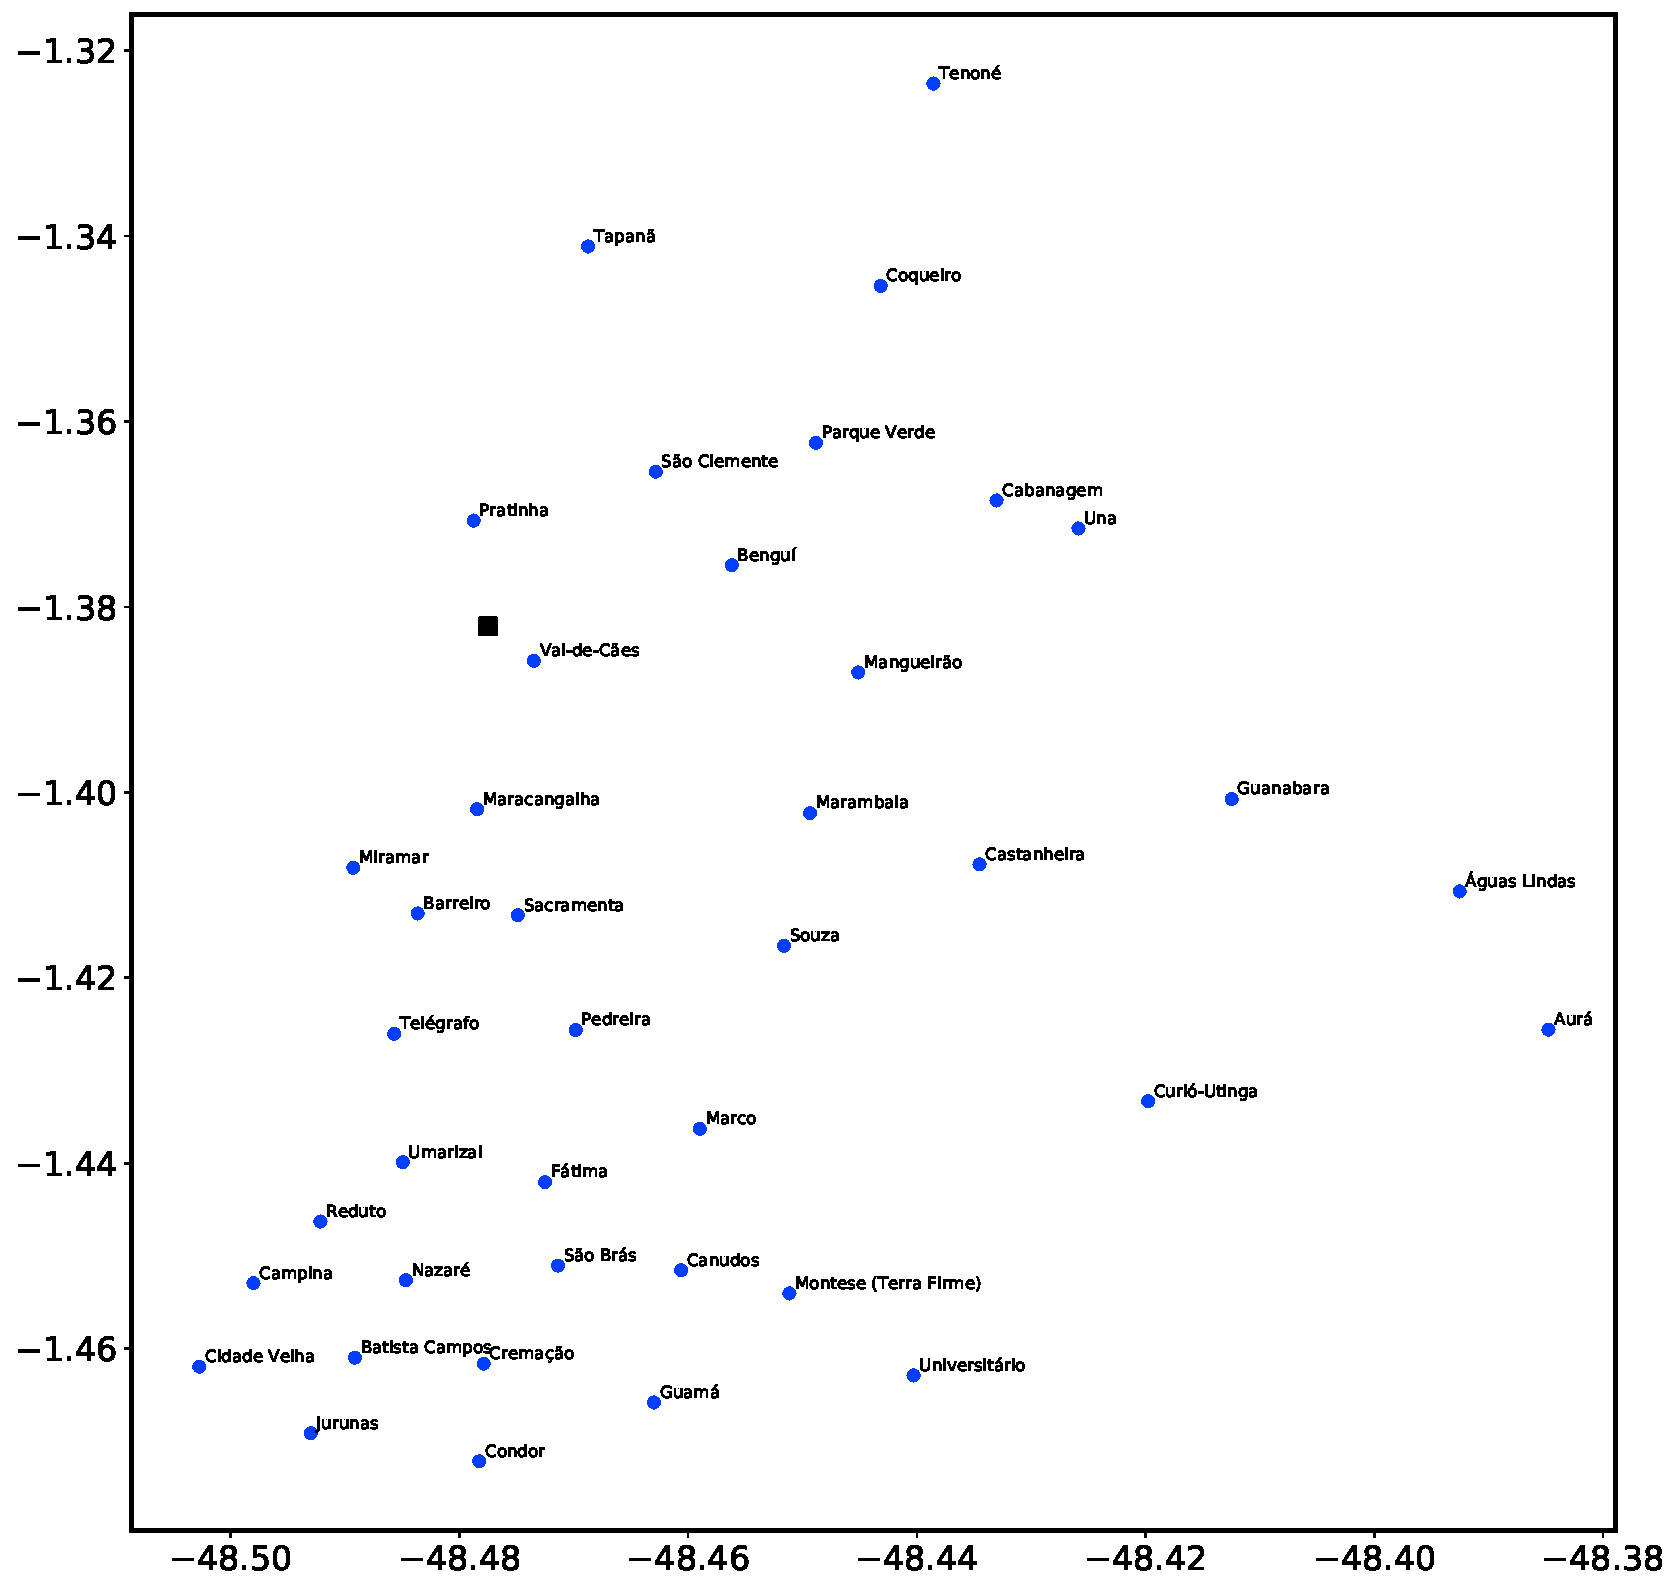
\includegraphics[width=\linewidth]{figures/base_de_dados}
    \caption{Conjunto de dados construído. Fonte: acervo próprio.}
    \label{fig:base_de_dados}
\end{figure} 



% ------------------------------- %
% Metodologia do trabalho         %
% ------------------------------- %
\section{Metodologia do trabalho} %
% ------------------------------- %
\label{sec:metodologia}           %
% ------------------------------- %



O trabalho foi dividido em três etapas: construção da base de dados, implementação do algoritmo e realização de experimentos, e escrita do artigo.

Para a construção da base de dados, inicialmente verificou-se a lista de bairros de Belém \cite{belemwiki}. Em seguida, buscou-se a coordenada de cada bairro utilizando a ferramenta Nominatin do projeto \textit{OpenStreetMap}, a qual fornece a delimitação e o ponto central dos bairros. Ao todo, 40 pontos centrais foram coletados e armazenados em uma planilha no formato \texttt{.csv}.

A implementação do algoritmo foi feita na linguagem \texttt{python}. Uma série de módulos foram utilizados na implementação, entre os quais podem-se nomear \texttt{dask}, \texttt{numba}, e \texttt{numpy}. \texttt{dask} foi utilizado para a paralelização dos experimentos ao criar um \textit{cluster} de \textit{workers}; \texttt{numba} foi utilizado para a compilação \textit{just-in-time} de várias funções em código de máquina, bem como a paralelização de laços \texttt{for} dentro das funções compiladas; e \texttt{numpy} foi utilizado como base para as operações realizadas sobre os dados.

Em termos do algoritmo utilizado, o algoritmo \textit{$K$-Means} foi implementado. A implementação desenvolvida pelo autores possui a particularidade de permitir a especificação de centroides fixos, i.e., centroides que não devem ser atualizados a despeito de serem considerados como parte da solução. Dois critérios de parada foram adotados: número máximo de iterações (definido por padrão como $200$) e não-alteração de rótulos de centroides entre iterações.

Os experimentos foram realizados da seguinte forma: uma função foi redigida para realizar $n$ execuções do algoritmo em paralelo. Esta função executa $n$ vezes uma segunda função de forma paralelizada. Esta segunda função instancia um objeto da classe \texttt{KMedias}, passa a ele o conjunto de dados criado a fim de que ele seja clusteriado e retorna uma tupla contendo a solução encontrada e a função-objetivo (denominada na \textit{codebase} como erro, uma vez que uma solução ótima minimiza esse valor). As especificações do trabalho requisitaram no mínimo $n = 20$; contudo, considerando o tamanho diminuto da base de dados e a rapidez da implementação realizada, optou-se por definir $n = 1000$.

% fonte do nominatim


% -------------------- %
% Resultados           %
% -------------------- %
\section{Resultados}   %
% -------------------- %
\label{sec:resultados} %
% -------------------- %



O algoritmo \textit{$K$-Means} foi implementado de forma bem-sucedida, e a implementação desenvolvida foi utilizada para a resolução do problema proposto. A \autoref{fig:resultados} expõe a melhor e a pior solução encontrada nas $1000$ execuções da implementação desenvolvida do algoritmo \textit{$K$-Means}. Uma análise dessas soluções expõe uma significativa discrepância na qualidade dos resultados em favor da melhor solução, uma vez que as distâncias entre as observações e os centroides foram minimizadas.

\begin{figure}[t!]
    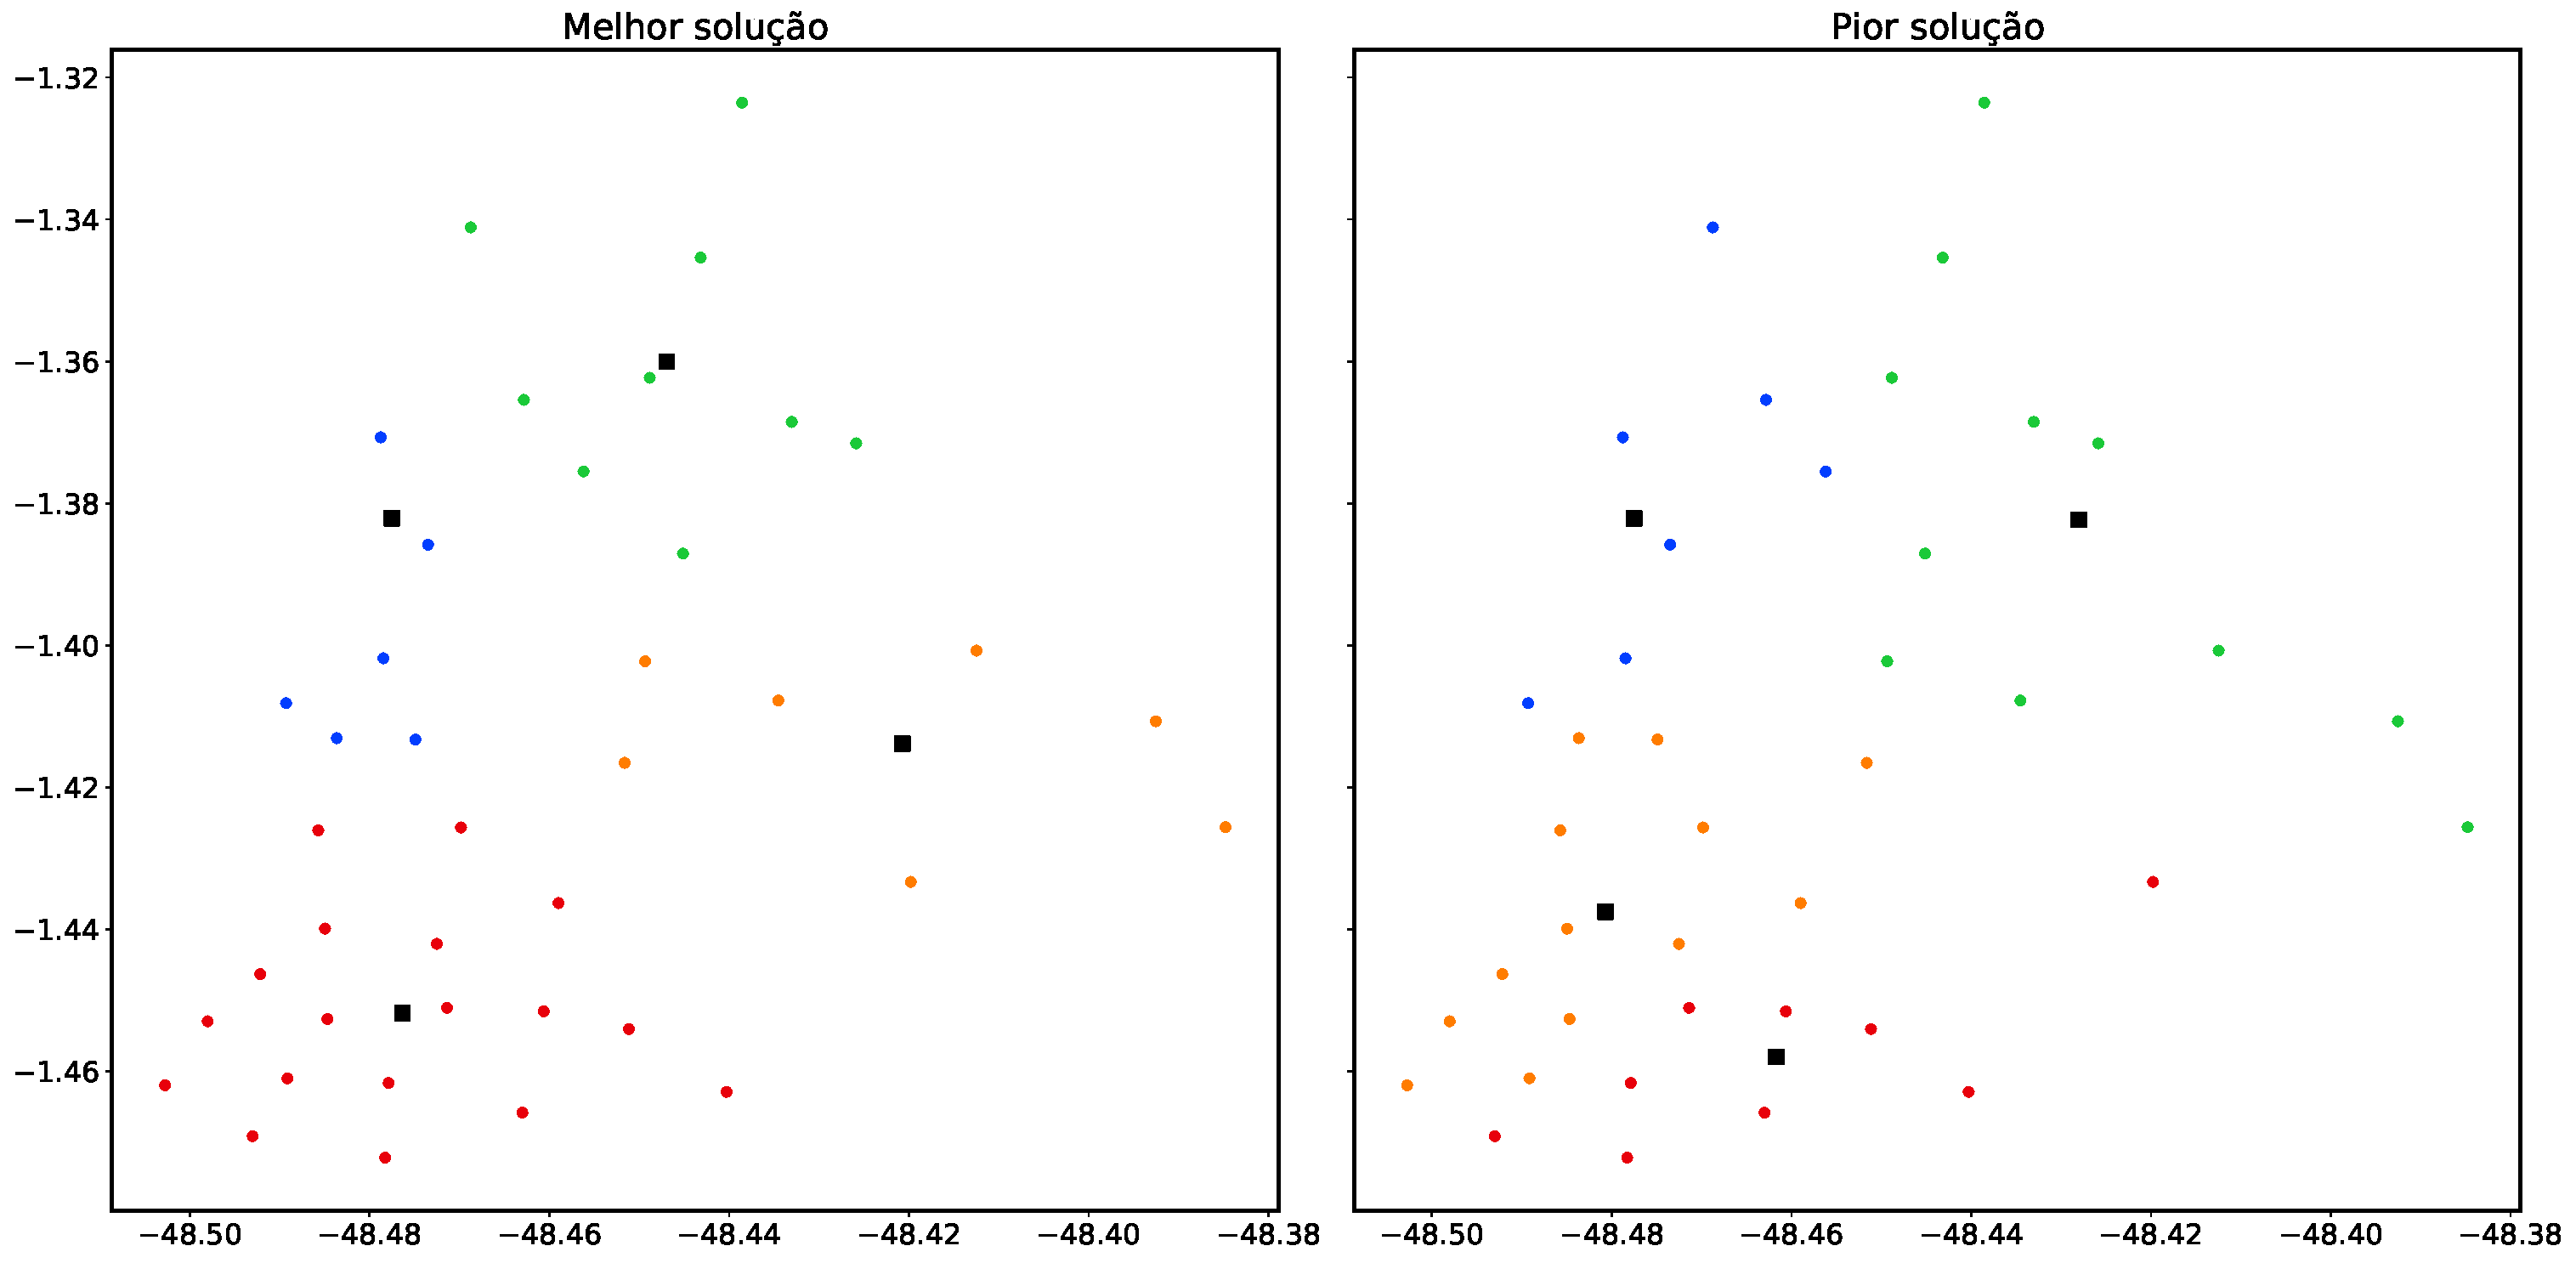
\includegraphics[width=\linewidth]{figures/resultados}
    \caption{Melhor e pior solução encontrada. Fonte: acervo próprio.}
    \label{fig:resultados}
\end{figure}

É importante observar como o \textit{cluster} azul, cujo centroide é o Aeroporto Internacional Val-de-Cans, permaneceu inalterado entre as duas soluções e o visto na \autoref{fig:base_de_dados}, o que comprova que o algoritmo não adulterou sua localização.

A \textit{codebase} desenvolvida registra todas as soluções encontradas, bem como seus erros, em um objeto \texttt{DataFrame}. Dessa forma, o usuário final pode verificar as demais soluções encontradas variando das melhores até as piores, a fim de auxiliar o processo de tomada de decisão em relação à melhor localização para os aeroportos.

Como produto adicional deste trabalho, tem-se que todas as funções desenvolvidas, bem como o conjunto de dados, seu pré-processamento, e seu processamento por meio da implementação desenvolvida do algoritmo \textit{$K$-Means}, foram consolidados em um arquivo \texttt{.ipynb}, i.e., em um Jupyter Notebook. Este arquivo encontra-se no repositório do GitHub \textbf{\href{https://github.com/ygarasab/kmeans}{@ygarasab/kmeans}}. Neste repositório, pode-se também consultar as contribuições realizadas por cada integrante desta equipe e auditar a implementação desenvolvida.


% ------------------- %
% Conclusão           %
% ------------------- %
\section{Conclusão}   %
% ------------------- %
\label{sec:conclusao} %
% ------------------- %



Com base no exposto acima, tem-se que o problema do aeroporto foi resolvido de forma
satisfatória pelo algoritmo \textit{$K$-Means}. A implementação desenvolvida se vale do módulo \texttt{numba} para compilação \textit{just-in-time} e paralelização de laços \texttt{for} a fim de tornar a execução do algoritmo tão rápida quanto possível e tirar máximo proveito da máquina em que é executado. Cumpre mencionar que todas as implementações produzidas foram desenvolvidas almejando total concordância com o estipulado no documento que descreve a atividade.

Em aderência ao requisitado nas especificações do trabalho e em reforço ao mencionado na \autoref{sec:resultados}, cumpre ressaltar que a ferramenta GitHub foi utilizada como sistema de versionamento no decorrer do desenvolvimento deste trabalho, de forma que as contribuições dos integrantes desta equipe possam ser registradas e vistas. Neste repositório, para além da \textit{codebase} desenvolvida para implementar o algoritmo \textit{$K$-Means}, foi criado um arquivo \texttt{.ipynb} (i.e., um Jupyter Notebook) consolidando todas as peças de código relevantes, executando os experimentos aqui descritos e expondo os resultados alcançados em mais detalhes. Todas essas contribuições adicionais podem ser encontradas em \textbf{\href{https://github.com/ygarasab/kmeans}{@ygarasab/kmeans}}.


% ------------------------- %
% Referências               %
% ------------------------- %
\bibliographystyle{sbc}     %
% ------------------------- %
\bibliography{sbc-template} %
% ------------------------- %

\end{document}
